% vim: spelllang=es

\chapter{Entendiendo Tremor}\label{ch:tremor}

\section{Sistemas de Procesado de Eventos}

Tremor es un \emph{Sistema de Procesado de Eventos}, que consiste en ``el
monitorizado y análisis (procesado) de flujos de información (datos) sobre cosas
que pasan (eventos)''~\cite{luckham2011event}. Tremor fue creado como una
alternativa de alto rendimiento a herramientas como \textcite{logstash} o
\textcite{telegraf}, pero ha evolucionado para soportar casos de uso más
complejos. Al contrario que esas piezas de software, Tremor también tiene
soporte para \emph{agregación} y \emph{rollups}, e incluye un lenguaje \emph{ad
hoc} para \emph{Extract, Transform, and Load (ETL)} y consultas.

Para más información sobre Tremor se puede consultar \textcite{tremorintro}, que
contiene una explicación de sus conceptos más básicos y sus posibles usos --- o
cuándo \emph{no} usarlo, en \textcite{tremorconstraints}.
\textcite{tremorrecipes} lista un total de 32 ejemplos de cómo configurar y
emplear el software.

La Figura~\ref{fig:tremor_example} ilustra uno de los casos de uso más básicos
de Tremor:

\begin{enumerate}
    \item Recibir \emph{logs} de varias aplicaciones en diferentes protocolos o
        formatos.
    \item Filtrar los casos redundantes, añadir campos y eliminar algunos
        innecesarios y transformar todo a un mismo formato.
    \item Enviar todos los logs estructurados a una base de datos para
        analizarlos posteriormente.
\end{enumerate}

\begin{figure}
    \centering
    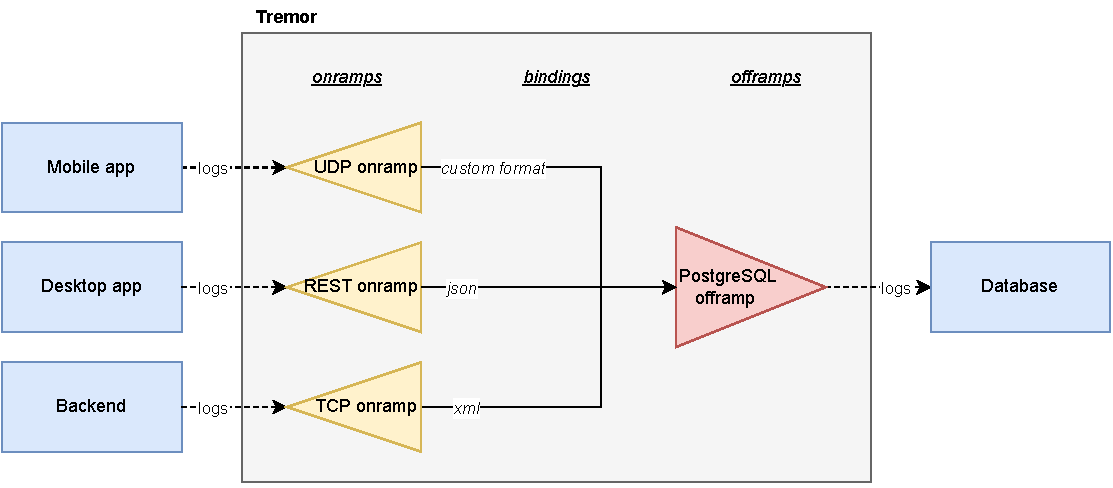
\includegraphics[width=\textwidth]{./Imagenes/example.pdf}
    \caption{Ejemplo de uso de Tremor}%
    \label{fig:tremor_example}
\end{figure}

Esto se basa en el concepto de \emph{onramps o sources} y \emph{offramps o
sinks}:

\begin{itemize}
    \item Una \onramp especifica cómo Tremor se conecta con el mundo exterior (o
        una \pipeline) para \textbf{recibir} de sistemas externos, como TCP,
        periódicamente, o PostgreSQL~\cite{tremoronramps}.

    \item Una \offramp especifica cómo Tremor se conecta con el mundo exterior
        (o una \pipeline) para \textbf{enviar} a sistemas externos, como
        \emph{stdout}, Kafka, o ElasticSearch~\cite{tremorofframps}.

    \item Una \pipeline es una lista de operaciones (transformación, agregación,
        eliminación, etc) a través de la cual se pueden encaminar los
        eventos~\cite{tremorpipelines}.

\end{itemize}

% TODO: explain 'artefacts', 'pre/postprocessors', 'codecs', 'operators'

Sin embargo, es posible que algunas \onramps no solo quieran recibir de sistemas
externos, sino también responderles directamente, actuando como una \offramp, y
viceversa. En la versión 0.11 --- la presente cuando me uní al proyecto --- este
problema se solucionaba con el concepto de \emph{linked transports}. Estos son
especialmente útiles para \onramps y \offramps como REST y \websockets, donde el
protocolo da la posibilidad de responder a eventos usando la misma conexión, por
ejemplo con un ACK.

El término \connector se introdujo en mayo con la versión 0.12. Solucionan el
problema desde el inicio, abstrayendo tanto los \onramps como los \offramps bajo
el mismo concepto, incluyendo los \emph{linked transports}. Dado que estos
estaban siendo desarrollados mientras 0.11 era la última versión, el sistema de
plugins se enfocó a \connectors, en lugar de \onramps u \offramps, que ahora
están en desuso.

A nivel de implementación, los \connector se definen con el \trait
\code{Connector}, que se puede simplificar a:

\begin{minted}{rust}
pub trait Connector {
    /// Crea la parte "source" del conector, si es aplicable.
    async fn create_source(
        &mut self,
        _source_context: SourceContext,
        _builder: source::SourceManagerBuilder,
    ) -> Result<Option<source::SourceAddr>> {
        Ok(None)
    }

    /// Crea la parte "sink" del conector, si es aplicable.
    async fn create_sink(
        &mut self,
        _sink_context: SinkContext,
        _builder: sink::SinkManagerBuilder,
    ) -> Result<Option<sink::SinkAddr>> {
        Ok(None)
    }

    /// Intenta conectarse con el mundo exterior. Por ejemplo, inicia la
    /// conexión con una base de datos.
    async fn connect(
        &mut self,
        _ctx: &ConnectorContext,
        _attempt: &Attempt
    ) -> Result<bool> {
        Ok(true)
    }

    /// Llamado una vez cuando el connector inicia.
    async fn on_start(&mut self, _ctx: &ConnectorContext) -> Result<()> {
        Ok(())
    }
    /// Llamado cuando el connector pausa.
    async fn on_pause(&mut self, _ctx: &ConnectorContext) -> Result<()> {
        Ok(())
    }
    /// Llamado cuando el connector continúa.
    async fn on_resume(&mut self, _ctx: &ConnectorContext) -> Result<()> {
        Ok(())
    }
    /// Llamado ante un evento de "drain", que se asegura de que no
    /// lleguen más eventos a este conector.
    async fn on_drain(&mut self, _ctx: &ConnectorContext) -> Result<()> {
        Ok(())
    }
    /// Llamado cuando el conector para.
    async fn on_stop(&mut self, _ctx: &ConnectorContext) -> Result<()> {
        Ok(())
    }
}
\end{minted}

Esencialmente, los plugins de tipo \connector exportarán esta interfaz de forma
pública en su binario, y la runtime deberá ser capaz de cargarlo de forma
dinámica. Actualmente, todos los \connectors disponibles se listan y cargan de
forma estática al inicio del programa.

Por tanto, es importante mantener la interfaz de plugins lo más simple posible.
Los detalles de comunicación deberían dejarse a la runtime, de forma que los
plugins se limiten a exportar una lista de funciones síncronas. De esta forma se
podrá evitar pasar tipos complejos (\code{async}, canales de comunicación, etc)
entre la runtime y los plugins, que implicaría una carga de trabajo mucho más
alta.

Una vez esta interfaz de bajo nivel se defina, podemos crear un \emph{wrapper}
en la runtime de más alto nivel (un \emph{manager}, en términos de Tremor) que
se encargue de la comunicación. Esto mismo lo hacen otras \crates como
\cratelink{rdkafka}, que implementa una capa de abstracción asíncrona sobre la
traducción directa de C en \cratelink{rdkafka-sys}.

\section{Funcionamiento interno}

Antes de comenzar a modificar el código existente en Tremor, es importante
conocer cómo funciona para evitar perder el tiempo. Tremor se basa en el modelo
actor. Citando Wikipedia:

% TODO: puedo hacer estas cosas? Me faltaría poner una citación a
% https://en.wikipedia.org/wiki/Actor_model al final del quote, pero así me
% ahorro explicarlo yo mismo.
``[The actor model treats the] actor as the universal primitive of concurrent
computation. In response to a message it receives, an actor can: make local
decisions, create more actors, send more messages, and determine how to respond
to the next message received. Actors may modify their own private state, but can
only affect each other indirectly through messaging (removing the need for
lock-based synchronization).''

No usa un lenguaje (e.g., Erlang) o framework (e.g., \cratelink{bastion}, quizá
en el futuro) que siga estrictamente este modelo, pero re-implementa los mismos
patrones frecuentemente de forma manual. Tremor se basa en \emph{programación
asíncrona}, es decir, que en vez de hilos trabajaremos con \emph{tareas}, un
concepto de nivel más alto. De la documentación de \cratelink{async-std}, la
runtime asíncrona que usa Tremor:

% TODO: faltaría referenciar
% https://docs.rs/async-std/1.10.0/async_std/task/index.html
``An executing asynchronous Rust program consists of a collection of native OS
threads, on top of which multiple stackless coroutines are multiplexed. We refer
to these as “tasks”. Tasks can be named, and provide some built-in support for
synchronization.''

Podríamos resumir su arquitectura con la frase ``Tremor se basa en actores
corriendo en tareas diferentes, que se comunican asíncronamente con canales''.
El actor principal se llama \code{World}. Contiene el estado del programa, como
los artefactos disponibles (\emph{repositorios}) y los que se están ejecutando
(\emph{registros}) y se usa para inicializar y controlar el programa.

Los \emph{managers} o \emph{gestores} son simplemente actores en el sistema que
envuelven una funcionalidad. Los gestores ayudan a desacoplar la comunicación y
la implementación de la funcionalidad interna. También son útiles para eliminar
código repetitivo al inicializar los componentes, así como la creación de
canales de comunicación, o el lanzamiento del componente en una tarea nueva.
Generalmente, hay un gestor por cada tipo de artefacto para ayudar con su
inicialización, y también un gestor por cada instancia que se esté ejecutando,
para controlar su comunicación.

Notar que la inicialización de los \connectors ocurre en dos pasos: primero se
\emph{registran}, es decir, indica que está disponible para cargarlo (y se añade
al repositorio). El \connector no empieza a ejecutarse hasta que se conecte con
otro artefacto con \code{launch_binding}, lo cual lo movería del repositorio al
registro, con el resto de artefactos ejecutándose.

A continuación se muestran los pasos que Tremor sigue para iniciar la ejecución
de un \connector, comenzando por el registro de un conector en la
Figura~\ref{fig:tremor_registering}.

\begin{figure}
    \centering
    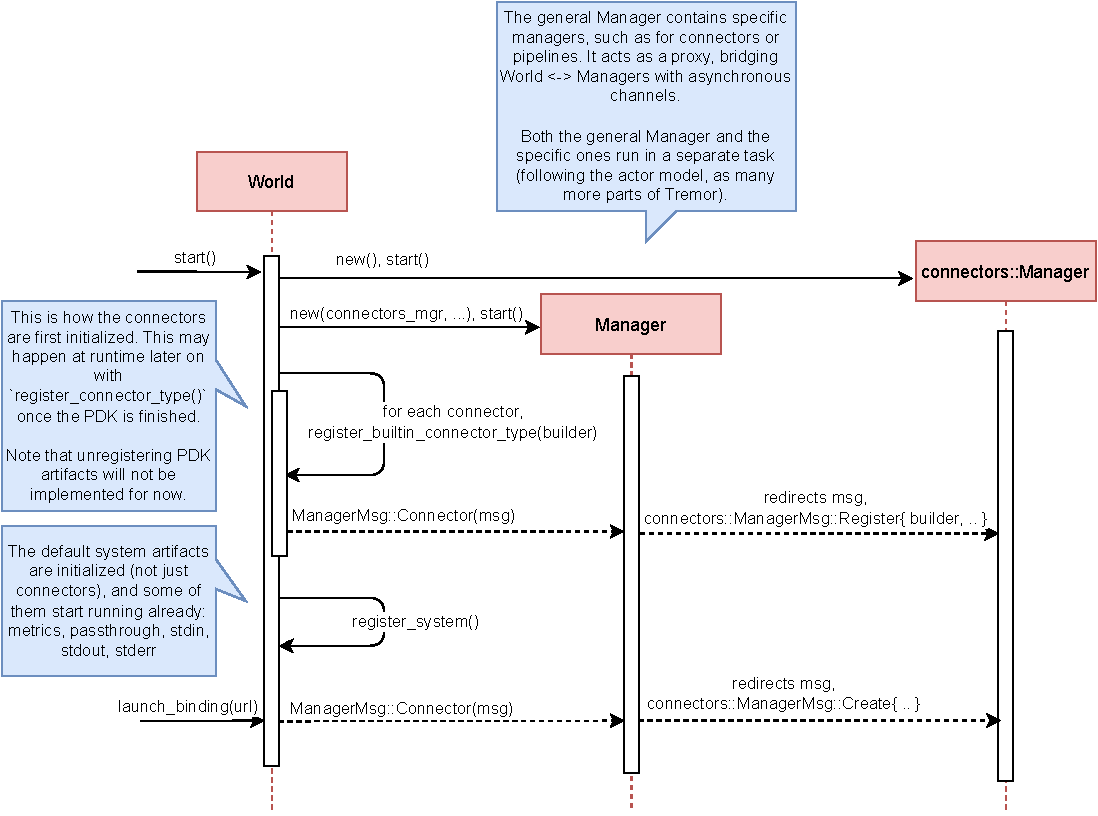
\includegraphics[width=\textwidth]{./Imagenes/registering.pdf}
    \caption{Registro de un conector en el programa}%
    \label{fig:tremor_registering}
\end{figure}

Una vez todos los gestores han sido inicializados, Tremor registra los
artifactos --- actualmente de forma estática con \code{register_builtin_types}.
Después de implementar el PDK, esto debería ocurrir dinámicamente, i.e., Tremor
buscaría automáticamente por archivos \code{dll}/\code{so} en su directorio
configurado, e intentaría registrar todos los plugins que encuentre. En una
futura versión, el usuario podría solicitar el cargado de un plugin nuevo
mientras se está ejecutando Tremor.

\code{connectors::Manager} contiene todos los conectores ejecutándose en Tremor,
que se muestra en la Figura \ref{fig:tremor_initializing}.

\begin{figure}
    \centering
    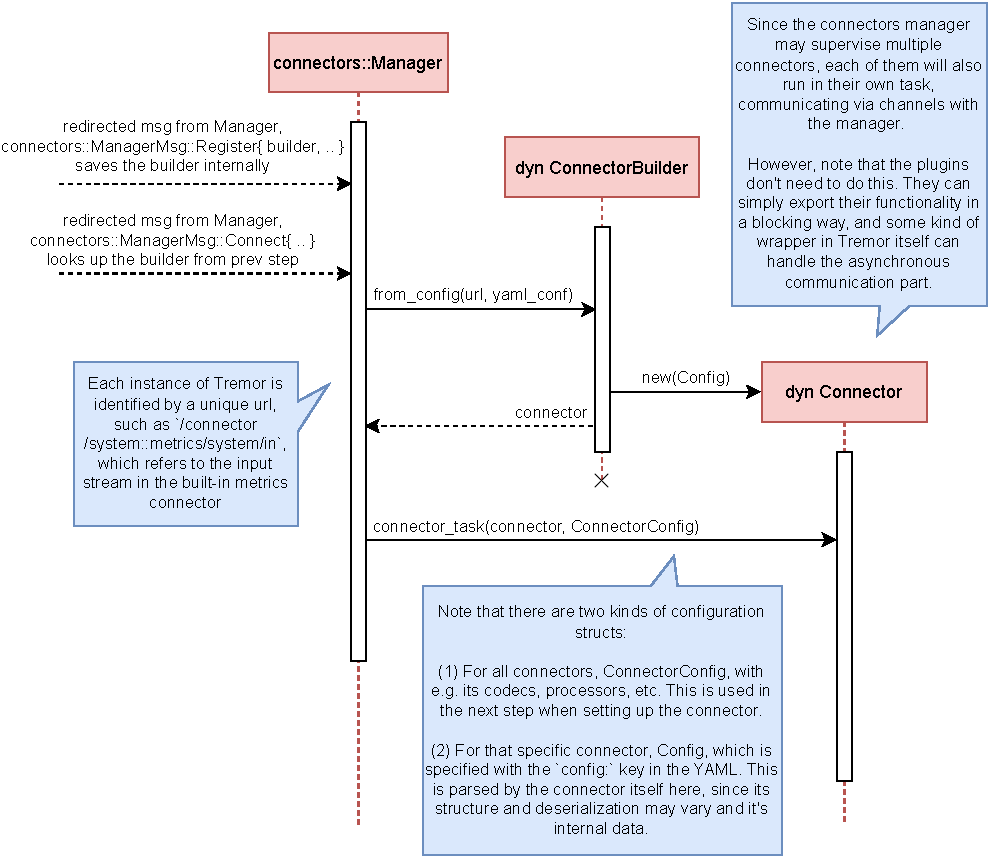
\includegraphics[width=\textwidth]{./Imagenes/initializing.pdf}
    \caption{Inicialización de un conector en el programa}%
    \label{fig:tremor_initializing}
\end{figure}

Ya que es un proceso en múltiples pasos (en la implementación es más complicado
que registro + creación), la primera parte provee las herramientas para
inicializar el conector (el \emph{builder}). Cuando el conector necesite
comenzar a ejecutarse porque se haya añadido a una \pipeline, el \builder ayuda
a construir y configurarlo de forma genérica. Finalmente, se añade a una tarea
propia para que se pueda comunicar con otras partes de Tremor.

Ahora que tenemos un \connector corriendo, visualizaremos cómo se divide en una
parte \sink y otra \source. De forma similar, un \builder se usa para
inicializar su \sink, \source, o ambos y posteriormente se inicia una nueva
tarea para ellos, como se puede observar en la Figura
\ref{fig:tremor_setting_up}.

\begin{figure}
    \centering
    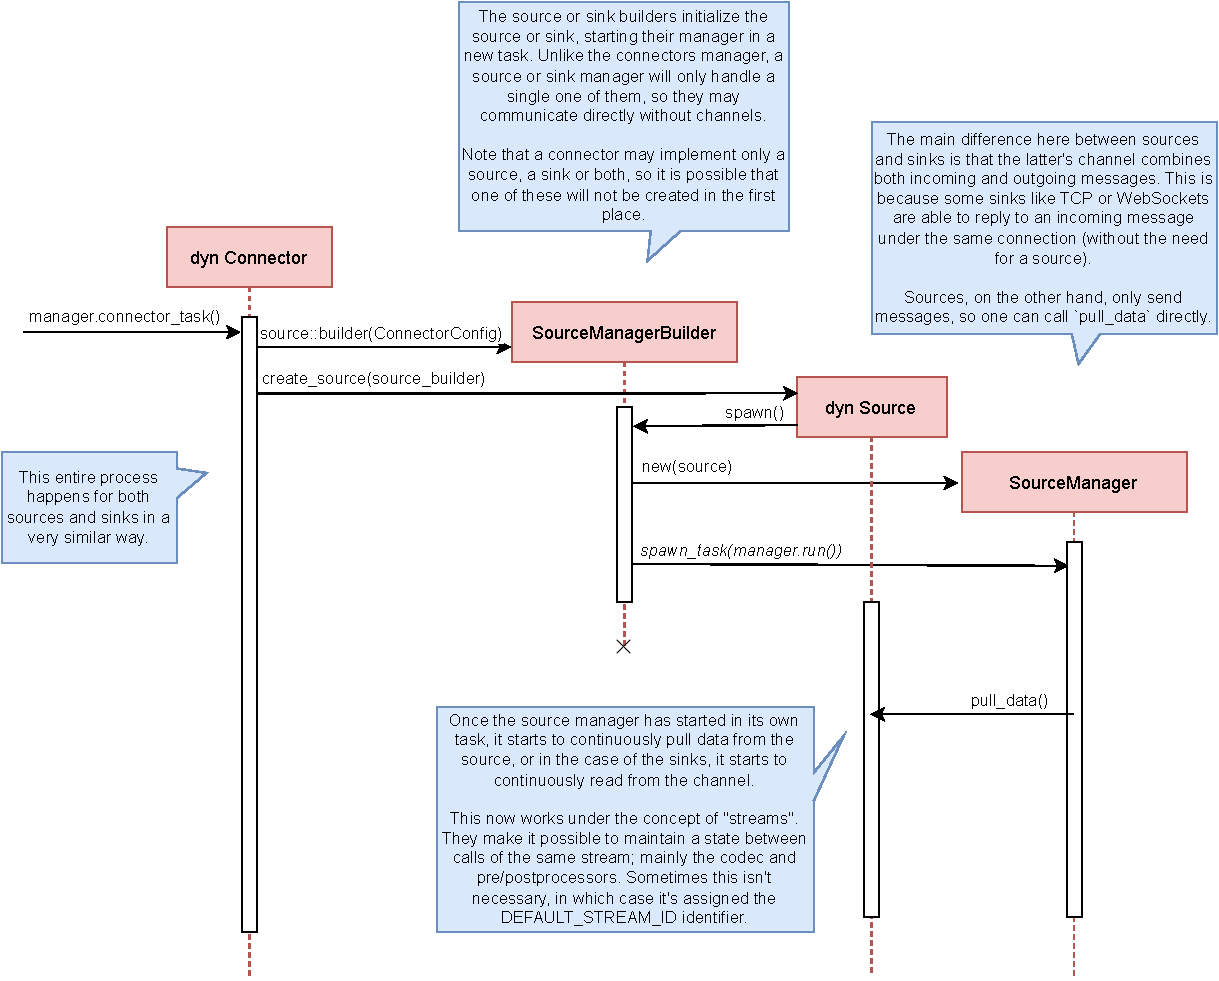
\includegraphics[width=\textwidth]{./Imagenes/setting-up.pdf}
    \caption{Configuración de un conector en el programa}%
    \label{fig:tremor_setting_up}
\end{figure}

También se crea un gestor por cada instancia de \sink o \source, que se
encargará de la comunicación con otros actores. De esta forma, sus interfaces
pueden mantenerse lo más simple posible. Esos gestores recibirán peticiones de
conexión de la \pipeline y posteriormente redirigirán o leerán de ella.

La diferencia principal entre \sources y \sinks a nivel de implementación es que
este último también puede responder a mensajes usando la misma conexión. Esto es
útil para notificar que el paquete ha llegado (\code{Ack}), o que algo ha
fallado (\code{Fail} para un evento específico, \code{CircuitBreaker}) para
dejar de recibir datos por completo.

Algunos conectores se basan en \emph{flujos}. Son equivalentes a los flujos de
TCP, que ayudan a agrupar mensajes para evitar mezclarlos. Se inician y
finalizan mediante mensajes, y el gestor se guarda su estado actual en un campo
llamado \code{states} (ya que, por ejemplo, algunos preprocesadores puedan
querer guardar un estado). Si un conector no necesita flujos, como
\code{metronome}, puede especificar su ID como \code{DEFAULT_STREAM_ID} siempre.

Los códecs y preprocesadores se involucran aquí tanto a nivel de \source como de
\sink. En la parte de \source, los datos son transformados a través de una
cadena de preprocesadores y posteriormente se aplica un códec. Para los \sinks,
se sigue el proceso inverso: los datos se codifican primero a bytes con el
códec, y posteriormente una serie de postprocesadores se aplican a los datos
binarios.

Después de implementar la interfaz de los conectores para el sistema de plugins,
podría escribir los siguientes plugins:

\begin{itemize}
    \item \emph{Blackhole}, usado para medir el rendimiento. Realiza mediciones
        de tiempos de final a final para cada evento pasando por la \pipeline, y
        al final guarda un histograma HDR (\emph{High Dynamic Range}).

    \item \emph{Blaster}, usado para repetir una serie de eventos de un archivo,
        que es especialmente útil para pruebas de rendimiento.

\end{itemize}

Ambos conectores son relativamente simples y serán de gran ayuda para realizar
\emph{benchmarks} para el PDK después. Sin embargo, lo más importante al
principio es que funcione, y después me encargaré del rendimiento.
